% ============================================================
%  CRD 中文稿（与 ICME 英文稿 CRD_ICME2027/ 同步，内部阅读版）
%  编译：xelatex main_cn.tex  × 2
%  数值与英文稿完全一致；英文稿某节改动后需手工同步本文件
% ============================================================
\documentclass[10pt,twocolumn,a4paper]{ctexart}

\usepackage[margin=1.9cm]{geometry}
\usepackage{amsmath,amssymb}
\usepackage{graphicx}
\usepackage{booktabs}
\usepackage{caption}
\usepackage[hidelinks]{hyperref}
\captionsetup{font=small,labelsep=quad}
\graphicspath{{../fig/}}

\setlength{\columnsep}{0.7cm}
\renewcommand{\figurename}{图}
\renewcommand{\tablename}{表}

\title{\bfseries CRD：面向全局图文错标检测的跨模态分数校准}
\author{}
\date{}

\begin{document}
\maketitle

\begin{abstract}
\noindent
网页规模图文数据的清洗，通常归结为对冻结视觉语言模型给出的相似度取阈值；这一操作的
前提是分数在不同图文对之间可比。本文检验该前提。在受控基准的 Attribute 维度上，
原始 CLIP 相似度把 $31.9\%$ 的 clean/noisy 组合排反，而同一编码器把两类样本分开的
能力远高于随机水平。我们把这一现象部分归因于可从图像与文本特征预测、且与「是否匹配」
基本无关的加性分数成分。据此提出 CRD：保持编码器冻结，在图像与文本特征之上拟合两个
小型加性头，再从一对图文对的标准化相似度中减去所估计的成分。两个头以逐对目标回归，
推理只需单独一对，不需要参考库、配对文本或 cycle；校准本身每对增加 $0.2$\,ms。
我们还构建了 FGBench——由 COCO 与 Visual Genome 的结构化事实冲突生成的
$88{,}024$ 个 reciprocal cycle，覆盖五个事实维度。在十五个基座—维度单元上，CRD 均改善
全局 clean/noisy 判别：CLIP ViT-B/16 的 Attribute AUROC 由 $0.6806$ 提升到 $0.7187$，
$24$ 项配对比较中 $21$ 项经 Holm 校正后仍显著；两种不含任何学习的特征去偏对照
（均值中心化余弦与 All-but-the-top 余弦）均未复现该增益，CRD 在五个维度上都优于二者。
本文同时界定方法边界：它不改善同图候选排序，在 Quantity 上也没有超过 CSLS。
\end{abstract}

\noindent\textbf{关键词：}\emph{图文错标；跨模态相似度；分数校准；视觉语言模型；数据清洗；评测基准}

% ============================================================
\section{引言}
% ============================================================

视觉语言模型已成为构建图文训练语料的标准工具：候选池被编码，每对获得一个相似度，
低于阈值的样本被丢弃或进入复标队列。同一分数还被复用于检索流水线，以及决定下游模型
能够见到哪些样本的数据清洗循环。这些用途共享一个前提——相似度可以\emph{跨对}比较，
即得 $0.33$ 的对子比得 $0.25$ 的对子更脏。本文考察该前提失效时会发生什么，并给出
一种低成本的修正。

现有检测方法或作用于编码器，或作用于邻域。有的用 CSLS 之类的 hubness 校正分数替换
余弦相似度，有的训练图文匹配头并对其输出取阈值，还有的借助最近邻或 reciprocal cycle
利用跨对结构。它们改善的都是随后被取阈值的\emph{信号}，却共同留下另一个问题：信号固定
时，两个互不相关的对子给出的数值是否处在同一尺度上？图~\ref{fig:mot1} 给出基准中
COCO 部分的一个反例：一个正确匹配的对子得 $0.252$，而一个把动物数量写错的 caption
所在的对子得 $0.331$。在同一冻结编码器下，错的那个以 $0.079$ 的优势胜出。

仅靠容量无法解决这一问题。全局检测与同图候选排序是两项不同的任务。候选排序的比较局限
在单张图内部，逐图偏移会相互抵消，更强的编码器几乎总是有帮助；全局检测的比较跨越图像与
文本，逐图与逐文本的贡献都进入决策。更强的编码器可能把两个分数同时抬高而保持其序，
这正是我们测到的：参数为 $427.6$M 的 CLIP ViT-L/14（ViT-B/16 为 $149.6$M）在
Attribute 上并未改变 AUROC（$0.6779$ 对 $0.6806$）。缺的不是容量，而是对「本不该进入全局比较的那部分分数」的
显式建模。

因此，我们把一对图文对的标准化相似度视为两项之和：一项承载跨模态匹配，另一项仅由图像
特征 $u$ 与文本特征 $v$ 即可预测。后者以加性形式建模，
$g_\theta(I,T)=a_\phi(u)+b_\psi(v)+b_0$，由两个小型头在每条图文对自身的标准化分数上
回归得到。推理时减去该估计量 $z' = z - \lambda g_\theta(I,T)$，所得分数在一对内部
保持单调，但不再携带可预测的逐模态成分。编码器始终不更新，两个头以 Huber 回归拟合每对
自身的标准化分数，$\lambda$ 在验证集上选取。推理只消费孤立的一对：没有参考库，没有
配对文本，没有 cycle。

我们在为该项任务构建的基准上评估上述方案。FGBench 包含 $88{,}024$ 个 reciprocal
cycle，源自 COCO 与 Visual Genome 的结构化事实冲突，覆盖 Entity、Quantity、
Attribute、Action 与 Relation 五个维度。每个 cycle 贡献两个匹配、两个不匹配的对子，
因此类别严格平衡，且每张图与每条文本各以一次匹配、一次不匹配出现。在五个冻结基座上，
校准分数均改善全局判别；消融显示两个头承载互补信息、逐对监督优于 cycle 均值监督、
打乱回归目标后增益完全消失。

\noindent\textbf{本文贡献。}
\begin{itemize}
  \item \textbf{方法}：CRD，一种事后校准方法。它在冻结编码器之上用两个轻量头估计
  图像侧与文本侧的加性分数成分，并从标准化相似度中扣除；在不引入任何推理期参考结构的
  前提下改善全局 clean/noisy 判别。
  \item \textbf{基准}：FGBench，包含 $88$k 个 reciprocal cycle、五个事实维度、
  明确的划分卫生与结构化审计流程，并开放对照方法在同一基座下的参考实现。
  \item \textbf{分析}：跨五个基座的评估，既报告增益也报告边界，包括带 Holm 校正的
  配对 bootstrap 检验、分离各项设计选择的消融，以及更简单的校正仍然更优的具体情形。
\end{itemize}

\begin{figure*}[t]
  \centering
  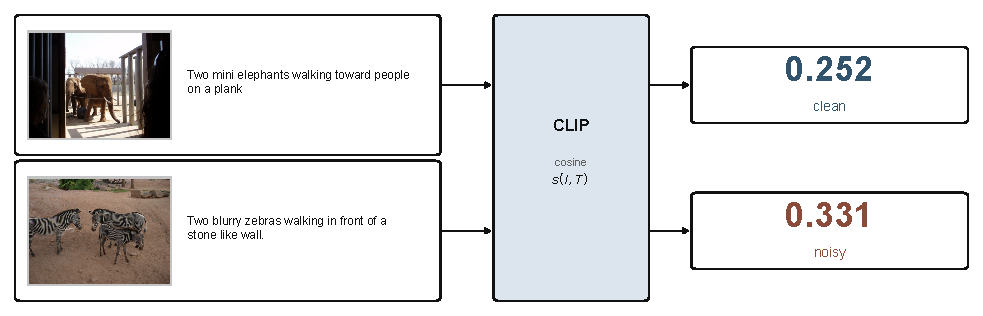
\includegraphics[width=\textwidth]{fig1_coco.pdf}
  \caption{原始图文相似度并不能把正确对子排在错误对子之上。两对均来自 COCO Quantity
  维度，由同一个冻结 CLIP ViT-B/16 打分，分数未作任何修改。上（正确匹配）为 $0.252$，
  下（数量写错）为 $0.331$。对原始分数取阈值会把两者判反。图像为 COCO 原图。}
  \label{fig:mot1}
\end{figure*}

% ============================================================
\section{相关工作}
% ============================================================

\subsection{图文匹配与错标检测}
CLIP~\cite{clip}、BLIP~\cite{blip}、SigLIP~\cite{siglip} 等对比式编码器把图像与文本映射到共享空间，余弦相似度是标准匹配
分数。在此之上的噪声检测沿三条路线展开。其一保留分数、改变其尺度：CSLS~\cite{csls} 之类的
hubness 校正变体用邻居集合重新规整每个分数，密度模型则拟合语料上的分数分布并对估计的
噪声率取阈值。其二用学习到的匹配器替换分数，通常是在同一编码器上训练的图文匹配头。
其三利用关系结构或文本自身的演化。LEMoN~\cite{lemon} 用多模态邻居给一对打分：
把候选 caption 与视觉近邻图像的 caption 比较、把图像与文本近邻 caption 所对应的图像
比较，从而相对于一个参考池判定该对是否有误。TRACED~\cite{traced} 则编辑 caption
本身，构造一条逐步改善的 caption 轨迹，并读取随之产生的相似度序列与语义变化。两者都
有效，但都把「是否有误」定义在该对自身分数之外。

三类方法对邻域的假设不同。基于邻居的校正需要推理时存在参考库、或批次内的其余对子，
其「一对是否有错」是相对于该集合而言的。本文的设定更严格：一对进、一个分数出，
不访问任何其他样本。

\subsection{视觉语言相似度与分数校准}
相似度分数在不同样本间不可直接比较，这在检索（hubness 与各向异性扭曲近邻排序）与
度量学习（分数校准是常规操作）中均已确立。先前工作从三个方向处理：用参考集重新规整
分数（CSLS 用邻居做逐侧减法即为一例）、对分数施加单调变换、或拟合分数的生成模型并对
后验取阈值。与 CRD 的关键区别不在于校正是否可加——CSLS 同样是加性校正——而在于校正量
的来源。CSLS 由参考库的统计量导出，并不针对当前这对的分数做拟合；本文的校正量由产生
该分数的那两个特征、在该对自身的标准化分数上回归得到，因而对孤立的一对也可用。分布层面
的重标定则另有区别：它作用于分数取值而不改变排序，这正是我们在实验中观察到的 GMM
基线的行为。

\subsection{细粒度图文评测基准}
FOIL~\cite{foil}、SugarCrepe~\cite{sugarcrepe} 等组合性基准给出一张图与一条正确 caption、一条被扰动的 caption，
度量模型是否偏好正确者。它们在同图二选一偏好下量化模型对某类语言扰动的敏感性，此时
逐图偏移会抵消。本文的基准关注另一个问题：给定两个互不相关的对子，哪个更脏。我们同时
报告跨对 AUROC 与同图 2AFC，正因为二者可能朝相反方向移动；实验显示 CRD 改善前者而
后者保持不变。

% ============================================================
\section{问题定义与动机}
\label{sec:problem-cn}
% ============================================================

\subsection{任务定义}
设 $f_I$、$f_T$ 为冻结的图像与文本编码器，$u=f_I(I)$、$v=f_T(T)$ 为对应特征。一对
图文对的原始分数取余弦相似度
\begin{equation}
  s(I,T)=\operatorname{sim}(u,v).
\end{equation}
每对带二值标签 $y\in\{0,1\}$ 表示 clean 或 noisy。任务是构造标量
$q(I,T)\in\mathbb{R}$，使得在测试集上按 $q$ 排序比按 $s$ 排序更能把 $y=1$ 与 $y=0$
分开。

两项性质把本任务与同图候选排序区分开。其一是\emph{全局性}：被排序的两对通常既不共享
图像也不共享文本。其二是\emph{对局部性}：$q(I,T)$ 不得依赖评测集中恰好还存在哪些其他
对子。相对于参考库给一对排序的方法违背第二条；只在单图内部重排候选的方法无法影响第一条。
因此我们把跨对 AUROC 与候选集内 2AFC 作为两个独立结果报告，而不合并为单一指标。

\subsection{原始相似度的经验局限}
图~\ref{fig:mot1} 给出 COCO Quantity 维度的一个例子：两对由同一冻结 CLIP ViT-B/16
打分，分数未作修改。正确匹配的一对得 $0.252$，数量写错的一对得 $0.331$。单个反例不足以
说明原始相似度不可靠，因此我们在改进空间最大的 Visual Genome Attribute 维度上做统计：
把全部 clean 对与 noisy 对两两比较，$31.9\%$ 的比较把 noisy 排在 clean 之上，等于该
维度的 $1-\mathrm{AUROC}$（$1-0.6806$）。图中所示 COCO Quantity 维度对应数值为
$16.9\%$（$1-0.8305$）。

同一效应也出现在单个 reciprocal cycle 内部（第~\ref{sec:fgbench-cn} 节），此时两张图
与两条 caption 均由构造固定。固定图像替换 caption 会改变分数（$0.324\to0.188$），
固定 caption 替换图像同样会改变（$0.324\to0.253$），四个值由同一编码器产生。可见分数
取决于「哪张图、哪条文本」，而非仅取决于二者是否对应；对该分数取阈值即把两件事混为
一谈。这两个比较属于图像条件与文本条件的分数变化，并不是对独立图像偏置或文本偏置的
测量，因为替换任一侧同时也改变了匹配本身。

\subsection{假设：加性分数成分}
设一对图文对的标准化分数可分解为
\begin{equation}
  z \;=\; \underbrace{m(I,T)}_{\text{跨模态匹配}} \;+\;
         \underbrace{c(I,T)}_{\text{加性成分}},
  \label{eq:decomp-cn}
\end{equation}
其中 $c$ 以可由 $u,v$ 预测的方式依赖两侧，且与二者是否对应基本无关。在
式~\eqref{eq:decomp-cn} 下，提升编码器抬高的是第一项，而不相关对子之间的序仍由第二项
支配，这与「更大的 CLIP 基座并未改变 Attribute AUROC」的观察一致。该分解也解释了单调
重标定为何无效：它作用于整体的 $z$，保留了两项共同诱导的排序。

式~\eqref{eq:decomp-cn} 是建模假设，而非关于分数如何生成的既定机制；我们也不声称 $c$
可被识别为图像噪声或文本噪声。被检验的是可操作推论：若 $z$ 中确有一部分可由 $u,v$
单独预测，则去除该预测应改善全局判别；而把预测拟合到置换后目标上的对照则不应改善。
第~\ref{sec:exp-cn} 节报告该检验。

% ============================================================
\section{跨模态分数校准}
\label{sec:method-cn}
% ============================================================

\subsection{概览}
本文将该流程称为 CRD，它是一种事后校准层：不修改任一编码器，在原特征之上增加两个小型头，
为单独一对返回校正后的分数。图~\ref{fig:overview-cn}(a) 为训练路径：一对图文对被编码为
$u,v$；两个特征同时进入加性头与相似度模块；两个头以该对自身的标准化相似度为回归目标。
图~\ref{fig:overview-cn}(b) 的推理路径复用相同编码器与相同头，通过一次减法把原始标准化
分数与估计成分结合。任何阶段都不更新编码器参数，推理路径也从不观察标签。

\begin{figure*}[t]
  \centering
  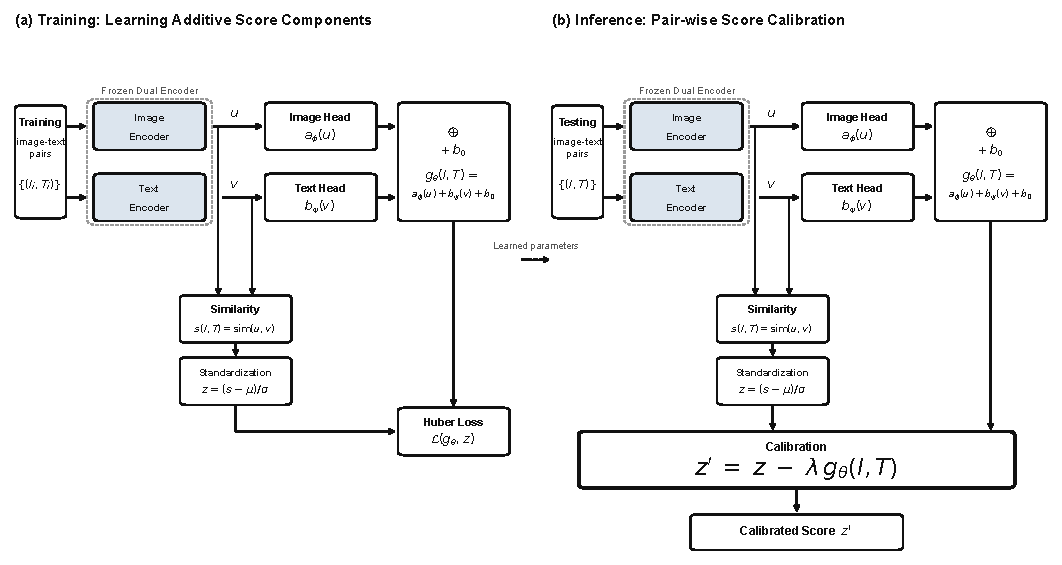
\includegraphics[width=\textwidth]{fig2_crd.pdf}
  \caption{CRD 框架总览。(a) 训练阶段：从\textbf{逐对}标准化的图文相似度中学习图像侧与
  文本侧加性成分；两个编码器冻结，仅优化两个头与偏置 $b_0$。(b) 推理阶段：从原始标准化
  相似度中减去估计的加性成分，得到校准后的成对分数；头与统计量 $\mu,\sigma$ 由训练固定，
  $\lambda$ 在验证集选取；只需一对，不需要参考库或 cycle。}
  \label{fig:overview-cn}
\end{figure*}

\subsection{冻结特征与分数标准化}
对一对 $(I,T)$ 计算
\begin{equation}
  u = f_I(I), \qquad v = f_T(T), \qquad s(I,T) = \operatorname{sim}(u,v),
\end{equation}
其中 $\operatorname{sim}$ 为余弦相似度。不同编码器的相似度尺度差异显著，故仅用训练集
估计统计量：
\begin{equation}
\begin{aligned}
  \mu &= \operatorname*{mean}_{(I,T)\in\mathcal{D}_{\text{train}}} s(I,T),\\
  \sigma &= \operatorname*{std}_{(I,T)\in\mathcal{D}_{\text{train}}} s(I,T) + 10^{-8},
\end{aligned}
\end{equation}
\begin{equation}
  z = \frac{s(I,T)-\mu}{\sigma}.
  \label{eq:z-cn}
\end{equation}
验证与测试对子使用同一组 $\mu,\sigma$；任何统计量都不在验证或测试集上计算。标准化有两重
作用：使同一套 $\lambda$ 网格在不同基座上有意义（原始分数范围可能相差一个数量级以上），
并使下一小节的回归目标与推理时扣除的残差处于同一尺度。

\subsection{加性分数估计}
估计成分为两个头的输出与一个偏置之和：
\begin{equation}
  g_\theta(I,T) \;=\; a_\phi(u) + b_\psi(v) + b_0,
  \label{eq:g-cn}
\end{equation}
其中 $a_\phi$ 为图像侧头，$b_\psi$ 为文本侧头，$b_0$ 为标量。每个头是含单隐层（宽度
$64$）与 GELU 非线性的两层感知机。这里保留加性形式而不在拼接特征上拟合联合残差网络：
联合网络的容量足以把匹配项 $m(I,T)$ 的一部分与目标成分一并吸收，而在本基准上加性形式
更强（第~\ref{sec:exp-cn} 节）。因此加性约束是由消融支持的设计选择，而非数学必然。

此处 $g_\theta$ 既不是第二个相似度，也不是对图像噪声或文本噪声的估计：它是标准化分数中
可由单侧特征预测的那一部分；下文所有结果均在这一解读下给出。

\subsection{逐对目标}
每条训练对贡献一个回归目标，即其自身的标准化分数 $z$：
\begin{equation}
  \mathcal{L}(\theta) \;=\; \frac{1}{|\mathcal{D}_{\text{train}}|}
  \sum_{(I,T)\in\mathcal{D}_{\text{train}}}
  \operatorname{Huber}\!\left(g_\theta(I,T),\, z(I,T)\right).
  \label{eq:loss-cn}
\end{equation}
以每对自身的分数、而非其 reciprocal cycle 的均值作为监督，是一个实质性选择：按构造，
cycle 内匹配与不匹配两条的 cycle 均值相同，用 cycle 均值作目标等于要求两个头预测一个在
「随后被排序的那组内部恒定」的量。第~\ref{sec:exp-cn} 节给出该差值为 $+0.62$\,pp AUROC，
逐对目标更优。

编码器冻结，仅优化 $\phi,\psi,b_0$。回归目标不涉及 clean/noisy 标签：头拟合的是分数而非
类别。标签只在选取 $\lambda$ 这一处进入；因此本方法并非完全无监督，本文也不如此描述。

\subsection{校准推理}
校准分数为
\begin{equation}
  \boxed{\,z' \;=\; z \;-\; \lambda\, g_\theta(I,T)\,}
  \label{eq:calib-cn}
\end{equation}
其中 $\lambda\ge 0$ 在验证集上按校准分数的 AUROC 选取：
\begin{equation}
\begin{aligned}
  \lambda^{\star} &= \arg\max_{\lambda\in\Lambda}\;
  \mathrm{AUROC}_{\text{val}}\!\left(z-\lambda\,g_\theta\right),\\
  \Lambda &= \{0,\,0.1,\,\dots,\,2.0\}.
\end{aligned}
\label{eq:lambda-cn}
\end{equation}
由于网格包含 $\lambda=0$，验证集可以判定无需校准；在安慰剂实验中它确实如此，此时校准
分数与原始分数重合。以 AUROC 而非回归损失选参是刻意的：所关心的是跨对排序，而不是
$g_\theta$ 对 $z$ 的拟合精度。

推理是对局部的：新来一对，特征编码一次，计算两个头，返回式~\eqref{eq:calib-cn}。不需要
参考库、配对文本、reciprocal cycle 或测试时阈值，这是与基于邻居的检测器最主要的实践差别。
额外开销为两次感知机前向，实测在 CLIP ViT-B/16 的 $15.1$\,ms 前向之上增加 $0.2$\,ms
（第~\ref{sec:exp-cn} 节）。

\subsection{训练协议}
两个头以 AdamW 优化 $1{,}500$ 次迭代，批大小 $256$，学习率 $10^{-3}$，权重衰减
$10^{-4}$，损失为默认转折点的 Huber。每个配置运行三个种子。训练子集、其行序以及由此
得到的 $\mu,\sigma$ 由固定数据种子决定，三次运行完全相同，仅初始化与批采样不同。每次
运行记录 manifest、特征缓存与行序的哈希并核验三者一致；该检查之所以存在，是因为按种子
抽取子集会把三个种子悄悄变成三个不同的数据集。第~\ref{sec:fgbench-cn} 节的 $2\times2$
构造是基准的性质，从不进入训练或推理。

% ============================================================
\section{FGBench 基准构建}
\label{sec:fgbench-cn}
% ============================================================

\subsection{设计原则}
FGBench 只回答一个问题——给定两个互不相关的对子，哪个更脏——其构造由该问题推出，而非由
语言覆盖度推出。五条原则指导设计：(i) 每张图与每条 caption 均为既有的 COCO 或 Visual
Genome 条目，不生成任何内容；(ii) 错标通过违反绑定于该图的结构化事实产生，使标签建立在
外部依据而非模型判断之上；(iii) 同一构造应用于五个事实维度，从而能报告检测器在何处有效、
在何处失效；(iv) 划分在 cycle 层面不相交，并核验训练与评测之间没有图像共享；(v) 构建
过程可审计：图~\ref{fig:mot1} 的定性样例中，图像内的物体计数、caption 陈述的计数与所赋
标签均经人工核对。

\subsection{Reciprocal cycle}
对选定的图像对 $(A,B)$ 及其 caption $(T_A,T_B)$，输出四条记录
\begin{equation}
\begin{aligned}
  &(A,T_A,\text{clean}),\quad (B,T_A,\text{noisy}),\\
  &(B,T_B,\text{clean}),\quad (A,T_B,\text{noisy}),
\end{aligned}
\end{equation}
构成一个 reciprocal cycle。该构造保证每张图与每条 caption 各以一次匹配、一次不匹配出现，
因此每个维度的类别比例按构造恰为 $50\%$，两类在图像侧与文本侧上的分布完全相同。它也消除
了朴素采样会带来的混杂：检测器无法利用某张图或某条 caption 的出现频率区分类别。

cycle 是数据的性质，不是方法的性质。CRD 在单条图文对上训练、对单独一对推理，从不消费
cycle。

\subsection{五个维度}
五个维度来自两个数据源。从 COCO 构建 \textbf{Entity}（替换物体类别）与
\textbf{Quantity}（替换数词）；从 Visual Genome 构建 \textbf{Attribute}（替换颜色、
材质或状态）、\textbf{Action}（替换谓词）与 \textbf{Relation}（替换空间或比较关系）。
Visual Genome 各维度均派生自 VG150 风格标注，本文称之为 VG150-derived 划分。

\subsection{数据统计}
\begin{table}[t]
\centering
\small
\setlength{\tabcolsep}{4pt}
\caption{FGBench v1-strict。每个 cycle 贡献两个匹配、两个不匹配对子，故每个维度严格平衡。
本文所有方法共用的测试划分包含 $17{,}565$ 个 cycle 与 $70{,}260$ 条对。}
\label{tab:fgbench-cn}
\begin{tabular}{llrr}
\toprule
来源 & 维度 & cycle 数 & 图文对 \\
\midrule
COCO & Entity & 32{,}589 & 130{,}356 \\
COCO & Quantity & 2{,}940 & 11{,}760 \\
Visual Genome & Attribute & 49{,}042 & 196{,}168 \\
Visual Genome & Action & 567 & 2{,}268 \\
Visual Genome & Relation & 2{,}886 & 11{,}544 \\
\midrule
\multicolumn{2}{l}{合计} & 88{,}024 & 352{,}096 \\
\bottomrule
\end{tabular}
\end{table}

表~\ref{tab:fgbench-cn} 汇总了构建规模：共 $88{,}024$ 个 cycle 与 $352{,}096$ 条图文对
记录，所有方法共享的固定测试划分包含 $17{,}565$ 个 cycle 与 $70{,}260$ 条对。

\subsection{标注协议与审计}
标签是 \emph{silver} 的：由替换规则作用于结构化标注得到，而非逐对人工裁定。该规则有已知
失效模式——标注记录的是「标注了什么」，并非图像的完整清单，因此提到一个物体的 caption
对同时包含其他物体的图像可能完全成立。为此，未标注内容被视为未知而非不存在，并为
Relation 保留严格层级，只保留标注支撑明确的样本；全文报告该严格层级（v1-strict）的结果。

所有检测器在完全相同的测试 manifest 上评测：我们核验每个方法的逐样本分数文件都解析到
相同的 $17{,}565$ 个 cycle，无法在全划分上评测的方法会被如实报告，而不会静默地在子集上
计分。

% ============================================================
\section{实验}
\label{sec:exp-cn}
% ============================================================

\subsection{实验设置}
\textbf{基座}：除特别说明外，所有方法共享同一个冻结 CLIP ViT-B/16，因此
表~\ref{tab:main-cn} 各行之间的差异来自检测器而非表示。第~\ref{sec:cross-cn} 节在另外
四个冻结编码器上重复比较：CLIP ViT-L/14、SigLIP2 以及 BLIP 的 ITC 与 ITM 两个变体。

\textbf{训练}：两个头按第~\ref{sec:method-cn} 节的协议优化（AdamW、$1{,}500$ 次迭代、
批大小 $256$）。每个配置运行三个种子，训练子集、行序与由此得到的 $\mu,\sigma$ 由固定数据
种子决定，三次运行仅初始化与批采样不同。每次运行记录 manifest、特征缓存与行序的哈希并
核验一致。

\textbf{指标}：主指标为跨对 AUROC，即全局检测器取阈值所面对的量；同时报告 AUPRC。2AFC
（同图候选对中偏好正确 caption 的比例）单独报告；它度量组合性基准所关注的性质，与 AUROC
不可互换。数值为三种子均值 $\pm$ 标准差，配对统计使用同批运行的逐样本分数。

\textbf{统计}：与各基线的比较使用以 cycle 为簇的配对 bootstrap（$1{,}000$ 次重采样，
重采样 cycle 而非行），并在全部 $24$ 项比较上做 Holm 校正。

\textbf{协议说明}：Action 维度的官方验证集仅含两个 cycle，不足以选取 $\lambda$。仅对该
维度，从训练 cycle 中划出 $20\%$（$399$ 中的 $80$）作为内部验证集；核验其与保留训练集
之间无图像共享，并仅用保留训练行重算 $\mu,\sigma$。测试划分（$166$ 个 cycle）完全未动。
该协议下的结果以 $\dagger$ 标注。

\subsection{与同基座检测器的比较}
表~\ref{tab:main-cn} 将 CRD 与余弦阈值、CSLS、GMM 密度检测器，以及邻域与 cycle 家族的
LEMoN-style 与 TRACED-style 复现进行比较。各行共享 CLIP ViT-B/16 与同一测试 manifest。
LEMoN 与 TRACED 是我们实现的复现（style reproduction），不是这两种方法的官方代码
\footnote{正式引用待补；复现遵循原文的任务定义，并随基准一并发布。}。

\begin{table*}[t]
\centering
\small
\setlength{\tabcolsep}{14pt}
\caption{共享 FGBench 测试集上的 AUROC，各行均为冻结 CLIP ViT-B/16。CRD 报告三种子均值
$\pm$ 标准差，单次运行的基线无标准差。$^\dagger$Action 使用内部验证集选取 $\lambda$
（第~\ref{sec:exp-cn} 节）。加粗为该列最优。}
\label{tab:main-cn}
\begin{tabular}{lccccc}
\toprule
方法 & Entity & Quantity & Attribute & Action$^\dagger$ & Relation \\
\midrule
CLIP 余弦 & 0.9991 & 0.8305 & 0.6806 & 0.5913 & 0.5413 \\
CLIP + CSLS & \textbf{0.9996} & \textbf{0.8882} & 0.6866 & 0.5869 & 0.5417 \\
GMM & 0.9991 & 0.8305 & 0.6806 & --- & 0.5413 \\
LEMoN-style & 0.9990 & 0.8495 & 0.6843 & 0.5964 & 0.5436 \\
TRACED-style & 0.9985 & 0.8412 & 0.6875 & 0.6102 & 0.5356 \\
均值中心化余弦 & 0.9989 & 0.8570 & 0.6790 & 0.5890 & 0.5389 \\
ABTT 余弦 & 0.9985 & 0.8481 & 0.6765 & 0.5394 & 0.5464 \\
\textbf{CRD（本文）} & 0.9995 & 0.8837 & \textbf{0.7187} & \textbf{0.6145} & \textbf{0.5530} \\
 & & \scriptsize$\pm$.0011 & \scriptsize$\pm$.0001 & \scriptsize$\pm$.0009 & \scriptsize$\pm$.0001 \\
\bottomrule
\end{tabular}
\end{table*}

三点值得分开看。Attribute 上增益最稳定：相对余弦提升 $3.81$ 点，相对包括 CSLS 在内的
所有基线提升 $3.12$–$3.81$ 点，且置信区间最窄（相对余弦为 $[3.72,3.96]$）。Quantity
的绝对增益更大（$+5.32$ 点），但该维度上 CSLS 已解释了其中大部分。Action 上 CRD 取得
最高点估计（$0.6145$ 对 TRACED 的 $0.6102$），差 $+0.43$\,pp，配对置信区间
$[-1.71,2.72]$，未通过 Holm 校正；因此在该维度主张与 TRACED 相当，而非优于。Quantity
与 Entity 上顺序反转：CSLS 略高（$0.8882$ 对 $0.8837$，$0.9996$ 对 $0.9995$），两项差异
均不显著，本文也不把 CRD 描述为全面更优。

$24$ 项配对比较中 $21$ 项经 Holm 校正后显著；三项例外正是上述三处：Entity 对 CSLS、
Quantity 对 CSLS、Action 对 TRACED。

表中另有两种\textbf{不含任何学习}的特征去偏基线，它们构成本文主张最直接的反证：
若把特征的一阶结构去掉就能取得增益，那么学习式加性头便没有独立价值。均值中心化余弦
把每个特征平移为其模态在训练集上的均值并重新归一化；ABTT 余弦在此之上再投影掉前 $k$
个主方向，$k\in\{1,2,4,8,16,32\}$ 按验证集 AUROC 逐维度选取（Entity、Quantity、
Attribute 取 $k{=}1$，Relation 取 $k{=}16$，Action 取 $k{=}32$）。二者都只在训练集上
拟合，且只在唯一的 image id 与 caption id 上估计统计量，不使用任何标签、不做梯度训练。

结果对本文有利，但并不夸张：两种去偏基线的最大收益出现在 Quantity（中心化相对余弦
$+2.65$ 点），仍远低于 CRD 的 $+5.32$ 点；在 Attribute 上二者都没有超过原始余弦
（$0.6790$、$0.6765$ 对 $0.6806$）。把与这两种基线的比较单独作为包含 $10$ 项检验的
家族做配对 bootstrap + Holm，CRD 在全部 $10$ 项上显著更优：相对中心化在
Attribute、Quantity、Action、Relation、Entity 上分别高 $4.00$、$2.78$、$2.55$、$1.41$、
$0.07$ 点，相对 ABTT 分别高 $4.26$、$3.67$、$7.51$、$0.67$、$0.10$ 点；最弱的一项是
Relation 对 ABTT（置信区间 $[-0.03,1.32]$）。因此增益来自学习到的加性头，而不是简单的
特征白化。Entity 上所有方法都在 $0.9985$ 以上，该维度 $0.07$ 点的显著差异不应被解读为
实际优势。

\subsection{跨基座评估}
\label{sec:cross-cn}
\begin{table}[t]
\centering
\small
\setlength{\tabcolsep}{3.5pt}
\caption{五个冻结基座上的 CRD（AUROC，$\Delta$ 以点为单位）。头与 $\lambda$ 按基座、按
维度分别重新拟合。BLIP 为检索微调模型，其 Quantity 属域内结果，不可与同列的零样本编码器
比较。}
\label{tab:cross-cn}
\begin{tabular}{llccc}
\toprule
基座 & 维度 & 原始 & CRD & $\Delta$ \\
\midrule
CLIP B/16 & Attribute & 0.6806 & 0.7187 & +3.81 \\
 & Relation & 0.5413 & 0.5530 & +1.17 \\
 & Quantity & 0.8305 & 0.8837 & +5.32 \\
CLIP L/14 & Attribute & 0.6779 & 0.7139 & +3.60 \\
 & Relation & 0.5420 & 0.5626 & +2.06 \\
 & Quantity & 0.8677 & 0.9282 & +6.05 \\
SigLIP2 & Attribute & 0.7026 & 0.7509 & +4.83 \\
 & Relation & 0.5578 & 0.5723 & +1.45 \\
 & Quantity & 0.8947 & 0.9254 & +3.07 \\
BLIP-ITC & Attribute & 0.7365 & 0.7803 & +4.38 \\
 & Relation & 0.5898 & 0.6163 & +2.65 \\
 & Quantity & 0.9766 & 0.9812 & +0.46 \\
BLIP-ITM & Attribute & 0.8207 & 0.8478 & +2.71 \\
 & Relation & 0.6467 & 0.6585 & +1.18 \\
 & Quantity & 0.9859 & 0.9880 & +0.21 \\
\bottomrule
\end{tabular}
\end{table}

表~\ref{tab:cross-cn} 在五个原始相似度尺度差异显著的冻结编码器上重复校准。十五个
「基座—维度」组合中，校准分数均优于原始分数：从接近饱和的 BLIP-ITM Quantity 的
$+0.21$ 点，到 CLIP ViT-L/14 Quantity 的 $+6.05$ 点。把该表读作编码器排名需注意两点：
每个基座有自己的头与 $\lambda$，因此结论是「校准可跨架构迁移」，而非「单个头可跨编码器
迁移」；两个 BLIP 模型经检索微调，其 Quantity 数值属域内结果，不可与同列的零样本编码器
比较。

同族内放大编码器并未改变 Attribute 上的排序：CLIP ViT-L/14 有 $427.6$M 参数，
ViT-B/16 为 $149.6$M（约 $2.9$ 倍），但后者得 $0.6806$、前者仅 $0.6779$。该效应依赖维度——在 Quantity 上更大的基座把原始分数
由 $0.8305$ 提升到 $0.8677$。因此规模并非无关，但它本身不足以解决改进空间最大的那个
维度上的全局排序问题。

\subsection{消融实验}
\begin{table}[t]
\centering
\small
\setlength{\tabcolsep}{5pt}
\caption{Visual Genome Attribute、CLIP ViT-B/16 上的消融，三种子均值。所有行共享同一
冻结特征、训练划分与 $\lambda$ 网格。}
\label{tab:ablation-cn}
\begin{tabular}{lccc}
\toprule
配置 & AUROC & AUPRC & $\Delta$ \\
\midrule
CLIP 余弦（基座） & 0.6806 & 0.6680 & --- \\
仅图像 $a_\phi(u)$ & 0.6944 & 0.6807 & +1.38 \\
仅文本 $b_\psi(v)$ & 0.6956 & 0.6904 & +1.50 \\
\textbf{加性（CRD）} & \textbf{0.7187} & \textbf{0.7177} & \textbf{+3.81} \\
cycle 均值目标 & 0.7125 & 0.7077 & +3.19 \\
打乱安慰剂 & 0.6806 & 0.6680 & 0.00 \\
\bottomrule
\end{tabular}
\end{table}

表~\ref{tab:ablation-cn} 分离各项设计选择。去掉任一侧的头会损失约三分之一的增益：仅图像
$0.6944$、仅文本 $0.6956$，加性形式为 $0.7187$。两个单独增益之和（$1.38+1.50=2.88$）
小于联合增益（$3.81$），缺口 $0.93$ 点，说明两侧承载互补信息而非重复信息。

以 cycle 均值替代每对自身分数损失 $0.62$ 点（$0.7125$ 对 $0.7187$），与
第~\ref{sec:method-cn} 节的论证一致。安慰剂对照在结构相同的头上使用置换后的 cycle 均值，
结果精确回到基线（$0.6806$，增益 $0.00$），说明改善来源于特征与分数之间的真实关系，而非
额外参数。在这些运行中验证集选中了 $\lambda=0$，即验证集自身判定所拟合的头没有校准价值；
与基线的相等因此是选参结果，而非巧合。

以 cycle 为簇的配对 bootstrap 确认上述排序：加性减仅图像 $+2.43$\,pp、减仅文本
$+2.31$\,pp、减 cycle 均值 $+0.62$\,pp、减安慰剂 $+3.81$\,pp，三个种子方向一致，
极差不超过 $0.15$\,pp。

\subsection{效率}
在单张 V100 上，对含 $6{,}000$ 个候选的库，CLIP ViT-B/16 前向加余弦打分为 $15.06$\,ms
每对，加 CRD 为 $15.89$\,ms（$5.5\%$ 开销）；CSLS 为 $15.27$\,ms。两个头共 $65{,}795$
参数，耗时 $0.205$\,ms。BLIP 上对应数值为 ITC $33.32\to33.94$\,ms、ITM
$54.42\to55.04$\,ms。与基于邻居的检测器不同，CRD 在推理时的代价不随库规模增长，因为头
只观察单独一对。

\subsection{校准改变什么、不改变什么}
\label{sec:analysis-cn}
本文报告的 2AFC 是一个\textbf{cycle 级别的组比较}：对每个 reciprocal cycle，比较两条
clean 记录分数之和与两条 noisy 记录分数之和。一个 cycle 内部，两侧使用同样的两张图与
同样的两条 caption，只是配对方式不同。对式~\eqref{eq:calib-cn} 在 cycle 内求和：

\begin{equation}
\begin{aligned}
\Delta' &= \Delta
- \lambda\Big[\textstyle\sum_{\text{clean}}(a+b+b_0)\\
&\qquad\quad - \textstyle\sum_{\text{noisy}}(a+b+b_0)\Big],
\end{aligned}
\end{equation}

其中 $\Delta$、$\Delta'$ 分别为校准前后「clean 之和减 noisy 之和」。方括号项恒为零，
因为两侧都包含 $a(u_A)+a(u_B)+b(v_A)+b(v_B)+2b_0$。因此\textbf{任何}加性校正
$a(u)+b(v)+b_0$ 都不改变该指标，与 $a$、$b$、$\lambda$ 的具体形式无关。CRD 的 2AFC
按构造即与余弦相等，我们在五个维度上以四位小数核实（Attribute $0.8282$、
Quantity $0.9649$、Entity 与 Action $1.0000$、Relation $0.6501$）；CSLS 同为加性校正，
不变量相同。

该不变性是\textbf{指标本身的性质}，而不是「校准无害」的证据；它也不外推到同图候选
比较——那种比较下只有固定侧对应的头会抵消。两种特征去偏基线从反面印证了这一点：
中心化与 ABTT 不是可分离的加性项，因而会改变该指标（ABTT 在 Attribute 上由 $0.8282$
降到 $0.8193$，在 Action 上由 $0.7831$ 降到 $0.6145$）。

只对分数做全局重标定的检测器，在 AUROC 或任何秩统计量上都与余弦无法区分。
表~\ref{tab:main-cn} 的 GMM 行与这一预期一致，可作 sanity check：凡定义的维度其 AUROC
都与余弦相同，因为单调变换必然如此。但其 2AFC 在 Attribute 与 Relation 上分别下降
$1.24$ 与 $3.51$ 点，提示一旦引入估计的噪声率，被取阈值的量不再是分数的单调函数。
两条观察合起来正是同时报告两个指标的理由：排序可以被保留，而分数作为候选集内比较的
可用性仍可能被破坏。

\subsection{任务边界}
我们也在 SugarCrepe~\cite{sugarcrepe} 上评估了 CRD，该基准由同图候选对构成，校准并未稳定改善该指标。
在同一张图内部，两个头之一会抵消，剩余修正很小，因此面向跨对可比性的方法在同图偏好
测试上能发挥的空间有限。

\subsection{加性解读的适用范围}
式~\eqref{eq:decomp-cn} 断言存在可预测的加性成分，并不声称该成分可被识别为图像偏置或
文本偏置。第~\ref{sec:problem-cn} 节讨论的 $2\times2$ 比较显示替换任一侧都会改变分数，
但它无法把模态特定偏移与匹配本身的变化分开，本文也不如此呈现。加性假设有两条可检验推论，
在本数据上均成立：两个头互补而非冗余；置换安慰剂完全消除增益。二者都不能证明真实的分数
生成过程是加性的；联合残差模型原则上可刻画式~\eqref{eq:g-cn} 无法表示的交互作用，而我们
尝试过的变体在本基准上均未做到。

\subsection{局限}
\textbf{标签是 silver 的。} 基准标签由替换规则作用于结构化标注得到。提到一个物体的
caption 对同时包含其他物体的图像并不必然为假，因此一部分 noisy 对子可视为可接受的描述。
严格的标注层级与对定性样例的人工核对缓解了该问题，但标签并非大规模人工裁定。

\textbf{Relation 绝对值仍然偏低。} 该维度最好 AUROC 为 $0.5530$，相对余弦提升 $1.17$ 点。
校准缩小了差距，但未使关系冲突变得可靠可检，本文不主张更强结论。

\textbf{并非所有汇总结果都提升。} Quantity 与 Entity 上 CSLS 仍领先于 CRD，Action 上
CRD 与 TRACED 统计上不可区分。该方法改善的是加性成分占分数变化较大时的全局判别，并未在
每个维度上压倒所有基线。

\textbf{方法消耗一个验证集。} $\lambda$ 在带标签的验证集上选取。两个头从不观察标签，
但整体方法并非无监督，$\lambda$ 的选取方式本身即属于所报告内容的一部分。

% ============================================================
\section{结论}
% ============================================================

全局 clean/noisy 检测预设两个互不相关的图文对可以在同一相似度尺度上比较。本文记录了该
预设在一个冻结编码器下失效的实例，并在受控基准上量化——Attribute 维度有 $31.9\%$ 的
clean/noisy 比较被排反——进而把其中一部分效应归因于可由图像与文本特征自身预测的分数
成分。CRD 用两个小型加性头在冻结编码器之上估计该成分，并从单独一对的标准化相似度中减去。
构造刻意保持最小：不训练编码器、不需要参考库、推理不需要配对文本，每对开销 $0.2$\,ms。

在覆盖五个事实维度、$88{,}024$ 个 reciprocal cycle 的 FGBench 上，该校准在十五个基座—维度
单元上均改善 AUROC，把 CLIP ViT-B/16 的 Attribute 由 $0.6806$ 提升到 $0.7187$，并使 2AFC
保持不变。消融把增益定位在两侧联合与逐对回归目标上，而非额外容量；置换对照则完全消除
增益，两种无需训练的特征去偏基线同样未复现该增益。同一批实验也界定了主张的边界：CSLS 在 Quantity 与 Entity 上仍领先，Action 上相对
TRACED 的差异不显著，关系冲突依然困难，标签仍是 silver 的。

两个方向自然延伸。其一，放宽分解形式，使其能表示两侧之间的交互作用，同时仍由特征可预测。
其二，在数据构建侧，让标签由人工裁定而非规则导出，从而让绝对值——而不只是方法之间的相对
顺序——值得信任。

% ============================================================
\begin{thebibliography}{99}
\small
\bibitem{clip} Radford A, Kim J W, Hallacy C, et al. Learning transferable visual models from natural language supervision. ICML, 2021.
\bibitem{blip} Li J, Li D, Xiong C, et al. BLIP: Bootstrapping language-image pre-training for unified vision-language understanding and generation. ICML, 2022.
\bibitem{siglip} Zhai X, Mustafa B, Kolesnikov A, et al. Sigmoid loss for language image pre-training. ICCV, 2023.
\bibitem{coco} Lin T Y, Maire M, Belongie S, et al. Microsoft COCO: Common objects in context. ECCV, 2014.
\bibitem{vg} Krishna R, Zhu Y, Groth O, et al. Visual Genome: Connecting language and vision using crowdsourced dense image annotations. IJCV, 2017.
\bibitem{csls} Conneau A, Lample G, Ranzato M A, et al. Word translation without parallel data. ICLR, 2018.
\bibitem{foil} Shekhar R, Pezzelle S, Klimovich Y, et al. FOIL: A dataset for learning to compose phrase grounding and referring expressions. ACL, 2017.
\bibitem{sugarcrepe} Hsieh C Y, Zhang J, Ma Z, et al. SugarCrepe: Fixing hackable benchmarks for vision-language compositionality. NeurIPS Datasets and Benchmarks, 2023.
\bibitem{lemon} Zhang H, Balagopalan A, Oufattole N, et al. LEMoN: Label error detection using multimodal neighbors. arXiv:2407.18941, 2024.
\bibitem{traced} Afriat G, Lucas R, Meng X, et al. Seeing what's wrong: A trajectory-guided approach to caption error detection. ICLR, 2026.
\end{thebibliography}

\end{document}
